


\subsection{Hybrid Cloud Achievement}


Comet has easy to use CLI allowing the use of Comet as infrastructure for virtual cluster management.


Cloudmesh has more functionality:
\begin{itemize}
\item Access hybrid clouds OpenStack, (EC2, AWS, Azure) Access
  concrete
\item infrastructure demonstrated usages of FutureSystems, Chameleon,
\item CloudLab, Cybera (CA) Once we get access: Bridges, Jetstream, ...
\item (EC2, AWS, Azure)
\end{itemize}
A user could use all of them

\subsection{Motivation}

Users are flexible and can chose the infrastructure most suitable for a particular problem while accessing them through the same client.  Switching from one infrastructure to another is simple while using templates and defaults

\begin{verbatim}
cm var cloud=jetstream / bridges / aws / ...
cm default cloud=$cloud
cm boot
\end{verbatim}

Rich Platform Stacks to Enable Reusable Virtual Cluster Templates

\begin{itemize}
\item Leverage from open source and proprietary services and tools
\item Pick the one most suitable
\item Integrate in DevOps
\item Make available through Cloudmesh launchers
\end{itemize}
cloudmesh launcher

Example:Install a Compute Node


\subsection{Virtual Clusters}

\begin{itemize}
\item Successful Early Operations
\item Developed a functional cloud environment leveraging:
\item Existing Rocks virtual cluster features
\item IU's FutureGrid experience and Cloudmesh client
\item Our ability to integrate with the standard HPC environment
\item Successfully deployed OSG virtual cluster
\item Virtual cluster used for CAIDA BGP Hackathon 2016
\item Hardening features
\item On ramping new groups
\item Pushing virtual cluster capability further into Comet
\item Excitement and caution
\item Developing cluster templates (Generic HPC cluster, Big Data) via Cloudmesh Launchers
\end{itemize}

\subsection{Other achievements}
\begin{itemize}
\item Pioneering XSEDE Cloud Allocation and Accounting
\item Virtual clusters use compute nodes as building blocks
\item Allocated based on compute SUs
\item Usage tracked based on compute SUs
\item XDMoD adding cloud utilization features via Open XDMoD
\item Builds on hardware resource utilization from TACC Stats
\item Needed for Comet, Jetstream, future XSEDE cloud systems
\item Need to have ongoing conversation with early users about \item reporting
\item Should projects report back like gateways?
\item Users, jobs, etc.?
\item Projects will likely need to track for subsequent XRACs \item regardless
\item After OSG, Many New Projects Ready to Begin
\item User-Customized HPC
\item High Performance Virtual Cluster Characteristics
\item What About Data?
\item Local storage
\item Can use Seagate SSDs for large VM images
\item Local (SDSC) network access same as compute nodes
\item We provide modest (TB) storage via NFS now
\item Working on secure access to Lustre
\item Accessing Virtual Cluster Capabilities
\end{itemize}



\subsection{What is next: Platforms}

\begin{itemize}
\item Example: NIST BigData Working group
\item Gather use case input from all stakeholders 
\item Derive Big Data requirements from each use case.
\item Analyze/prioritize a list of challenging general requirements that may delay or prevent adoption of BigData deployment 
\item Work with Reference Architecture to validate requirements and reference architecture
\item Develop a set of general patterns capturing the {\em essence} of use cases (to do)
\item Rich Platform Stacks to Enable Reusable Virtual Cluster Templates
\item Leverage from open source and proprietary services and tools
\item Pick the one most suitable
\item Integrate in DevOps
\item Make available through Cloudmesh launchers
\end{itemize}

\subsection{Comet Cloudmesh Platform Launchers}

\begin{itemize}
\item Launch specific platform selections
\item Target Application user communities
\item Make deployment and management simple
\item Customizable launchers
\item Launchers available through commandline or browser
\item Underlying ZFS layer makes cloning cluster template trivial
\item Comet Cloudmesh Platform Launchers (Future)
\item Specific Launch
\item List of Launchers
\item Concepts, Ideas, Design
\end{itemize}

\subsection{Enabling Technologies}
\begin{description}
\item[KVM:] Let us run virtual machines (all processor features)
\item[SR-IOV:] Makes MPI go fast on VMs
\item[Rocks:] Systems management
\item[ZFS:] Disk image management
\item[VLANs:] Isolate virtual cluster management network
\item[pkeys:] Isolate virtual cluster IB network
\item[Nucleus:] Coordination engine (scheduling, provisioning, status,
  etc.)
\item[Cloudmesh:] The client to virtual cluster management is
  provided by cloudmesh 
\end{description}


\section{NIST Big Data Use Cases}

51 NIST Big Data Benchmark Detailed Use Cases

\subsection{Government Operation} 

National Archives and Records Administration, Census BureauCommercial:
Finance in Cloud, Cloud Backup, Mendeley (Citations), Netfilx, Web
Search, Digital Materials, Cargo shipping (as in UPS)Defense: Sensors,
Image surveillance, Situation AssessmentHealthcare and

\subsection{Life Sciences} 

Medical records, Graph and Probabilistic analysis, Pathology,
Bioimaging, Genomics, Epidemiology, People Activity models,
BiodiversityDeep Learning and Social Media: Driving Car, Geolocate
images/cameras, Twitter, Crowd Sourcing, Network Science, NIST
benchmark datasets

\subsection{The Ecosystem for Research} 

Metadata, Collaboration, Language Translation, Light source
experiments

\subsection{Astronomy and Physics} 

Sky Surveys compared to simulation, Large Hadron Collider at CERN,
Belle Accelerator II in JapanEarth,

\subsection{Environmental and Polar Science} 

Radar Scattering in Atmosphere, Earthquake, Ocean, Earth Observation,
Ice sheet Radar scattering, Earth radar mapping, Climate simulation
datasets, Atmospheric turbulence identification, Subsurface
Biogeochemistry (microbes to watersheds), AmeriFlux and FLUXNET gas
sensors

\subsection{Energy} 

SmartGrid infrastructure for virtual cluster management.



\begin{verbatim}
http://cloudmesh.github.io/client/reference_card.html#refcard-comet
http://cloudmesh.github.io/client/commands/command_comet.html#comet-command
\end{verbatim}


\subsection{Client Portal}

\begin{figure}[htb] 
  \centering 
    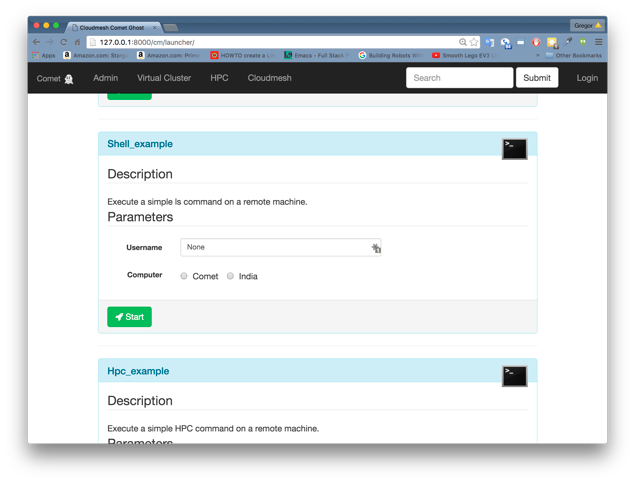
\includegraphics[width=1.0\columnwidth]{images/client/Picture6.png} 
    \caption{Virtual cluster launch parameters}
    \label{F:6}
\end{figure} 

\begin{figure}[htb] 
  \centering 
    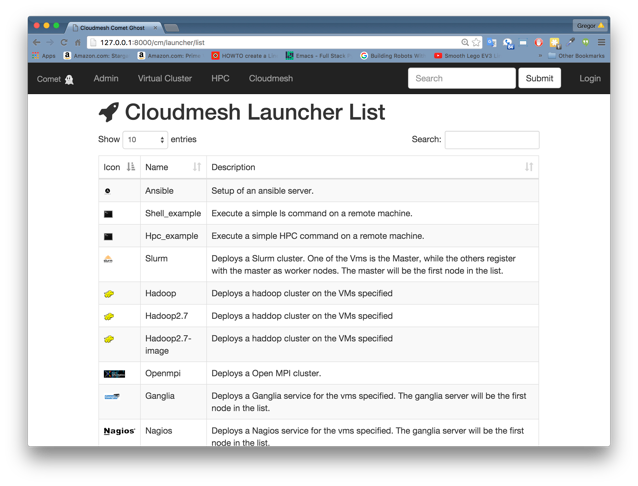
\includegraphics[width=1.0\columnwidth]{images/client/Picture7.png} 
    \caption{Virtual cluster launcher}
    \label{F:7}
\end{figure} 


\subsection{Form Tutorial}

\begin{figure*}[htb] 
\begin{small}
\begin{verbatim}

+------+---------+-------+------------------------------------------+---------------+------------+-----------+-------------+
| Name | Project | Count | Nodes                                    | Frontend (Fe) | State (Fe) | Type (Fe) | Description |
+------+---------+-------+------------------------------------------+---------------+------------+-----------+-------------+
| vc1  | sys200  | 8     | vc1-[0-7]                                | vc1           | nostate    | VM        |             |
| vc2  | iu      | 8     | vm-vc2-[0-7]                             | vc2           | active     | VM        |             |
| vc3  | sys200  | 16    | compute-0-[0-12,14],compute_windows_10,d | vc3           | active     | VM        |             |
|      |         |       | imm_dev_node                             |               |            |           |             |
| vc4  | iu      | 8     | tstfw[1-2],vm-vc4-[0-5]                  | vc4           | active     | VM        |             |
| vc5  | sys200  | 11    | vm-vc5-[0-10]                            | vc5           | nostate    | VM        |             |
| vc6  | rocks   | 8     | vm-vc6-[0-7]                             | vc6           | nostate    | VM        |             |
| vc8  | sys200  | 0     |                                          | vc8           | active     | VM        |             |
| osg  | osg     | 34    | vm-osg-[0-33]                            | osg           | active     | VM        |             |
+------+---------+-------+------------------------------------------+---------------+------------+-----------+-------------+
\end{verbatim}
\end{small}
\end{figure*}

\begin{figure*}[htb] 
\begin{small}
\begin{verbatim}

Comet Cloudmesh Client (cluster view)
(COMET)host:client$ cm comet cluster
Cluster: osg	Frontend: osg	IP: 10.21.255.180
Cluster: vc1	Frontend: vc1	IP: 10.21.255.182
.........
Cluster: vc8	Frontend: vc8	IP: 10.21.255.175
\end{verbatim}
\end{small}
\end{figure*}

\begin{figure*}[htb] 
\begin{small}
\begin{verbatim}


+--------------------+---------------+----------+------+-------------------+------+---------+--------+---------+------------+
| name               | state         | kind     | type | mac               | cpus | cluster | RAM(M) | disk(G) | computeset |
+--------------------+---------------+----------+------+-------------------+------+---------+--------+---------+------------+
| osg                | active        | frontend | VM   | ca:5f:a8:00:00:1b | 8    | osg     | 32768  | 36      |            |
|                    |               |          |      | ca:5f:a8:00:00:1c |      |         |        |         |            |
| vm-osg-0           | active        | compute  | VM   | ca:5f:a8:00:00:1d | 24   | osg     | 120000 | 100     | 1065       |
| vm-osg-1           | active        | compute  | VM   | ca:5f:a8:00:00:1e | 24   | osg     | 120000 | 100     | 1066       |
| vm-osg-2           | active        | compute  | VM   | ca:5f:a8:00:00:1f | 24   | osg     | 120000 | 100     | 1067       |
.........
| vm-vc6-6           | nostate       | compute  | VM   | ca:5f:a8:00:00:7a | 24   | vc6     | 120000 | 36      |            |
| vm-vc6-7           | nostate       | compute  | VM   | ca:5f:a8:00:00:7b | 24   | vc6     | 120000 | 36      |            |
| vc8                | active        | frontend | VM   | ca:5f:a8:00:00:6d | 2    | vc8     | 4096   | 160     |            |
|                    |               |          |      | ca:5f:a8:00:00:6e |      |         |        |         |            |
+--------------------+---------------+----------+------+-------------------+------+---------+--------+---------+------------+
\end{verbatim}
\end{small}
\end{figure*}

\begin{figure*}[htb] 
\begin{small}
\begin{verbatim}


Comet Cloudmesh Client (computeset view)
(COMET)host:client$ cm comet computeset --cluster=osg

ClusterID: osg	ComputesetID: 1065	 State: running		Allocation: sys200
Start (est): 03/29/16 16:55 EDT		End (est): 03/31/16 16:55 EDT
Requested Time (ddd-hh:mm): 2-00:00	Running Time (est): 1-19:23		Remaining Time (est): 04:36
+----------+--------+------+-------------------+------+---------+------+--------+
| name     | state  | type | mac               | cpus | cluster | host | memory |
+----------+--------+------+-------------------+------+---------+------+--------+
| vm-osg-0 | active | VM   | ca:5f:a8:00:00:1d | 24   | osg     |      | 120000 |
+----------+--------+------+-------------------+------+---------+------+--------+
\end{verbatim}
\end{small}
\end{figure*}

\begin{figure*}[htb] 
\begin{small}
\begin{verbatim}

ClusterID: osg	ComputesetID: 1066	 State: running		Allocation: sys200
Start (est): 03/29/16 17:00 EDT		End (est): 03/31/16 17:00 EDT
Requested Time (ddd-hh:mm): 2-00:00	Running Time (est): 1-19:17
Remaining Time (est): 04:42

+----------+--------+------+-------------------+------+---------+------+--------+
| name     | state  | type | mac               | cpus | cluster | host | memory |
+----------+--------+------+-------------------+------+---------+------+--------+
| vm-osg-1 | active | VM   | ca:5f:a8:00:00:1e | 24   | osg     |      | 120000 |
+----------+--------+------+-------------------+------+---------+------+--------+
\end{verbatim}
\end{small}
\end{figure*}

\begin{figure*}[htb] 
\begin{small}
\begin{verbatim}


Comet Cloudmesh Client (start new computeset)
(COMET)host:client$ cm comet start vc2 --count=2 --walltime=3h
Request accepted! Check status with:
comet cluster vc2
or:
comet computeset 1102
(COMET)host:client$ cm comet computeset 1102

(COMET)host:client$ cm comet start vc4 vm-vc4-[0,1] --walltime=1h
Request accepted! Check status with:
comet cluster vc4
or:
comet computeset 1103

ClusterID: vc2	ComputesetID: 1102	 State: running		Allocation: sys200
Start (est): 03/31/16 12:21 EDT		End (est): 03/31/16 15:21 EDT
Requested Time (ddd-hh:mm): 03:00	Running Time (est): 00:00		Remaining Time (est): 02:59

+----------+---------+------+-------------------+------+---------+------+--------+
| name     | state   | type | mac               | cpus | cluster | host | memory |
+----------+---------+------+-------------------+------+---------+------+--------+
| vm-vc2-3 | nostate | VM   | ca:5f:a8:00:00:16 | 24   | vc2     |      | 1024   |
| vm-vc2-2 | nostate | VM   | ca:5f:a8:00:00:15 | 24   | vc2     |      | 1024   |
+----------+---------+------+-------------------+------+---------+------+--------+
\end{verbatim}
\end{small}
\end{figure*}

\begin{figure*}[htb] 
\begin{small}
\begin{verbatim}

Comet Cloudmesh Client (cluster view for status check)
(COMET)host:client$ cm comet cluster vc2
Cluster: vc2	Frontend: vc2	IP: 10.21.255.181

+----------+---------+----------+------+-------------------+------+---------+--------+---------+------------+
| name     | state   | kind     | type | mac               | cpus | cluster | RAM(M) | disk(G) | computeset |
+----------+---------+----------+------+-------------------+------+---------+--------+---------+------------+
| vc2      | active  | frontend | VM   | ca:5f:a8:00:00:11 | 1    | vc2     | 1024   | 36      |            |
|          |         |          |      | ca:5f:a8:00:00:12 |      |         |        |         |            |
| vm-vc2-0 | active  | compute  | VM   | ca:5f:a8:00:00:13 | 24   | vc2     | 1024   | 36      | 1101       |
| vm-vc2-1 | active  | compute  | VM   | ca:5f:a8:00:00:14 | 24   | vc2     | 1024   | 36      | 1101       |
| vm-vc2-2 | active  | compute  | VM   | ca:5f:a8:00:00:15 | 24   | vc2     | 1024   | 36      | 1102       |
| vm-vc2-3 | active  | compute  | VM   | ca:5f:a8:00:00:16 | 24   | vc2     | 1024   | 36      | 1102       |
| vm-vc2-4 | nostate | compute  | VM   | ca:5f:a8:00:00:17 | 24   | vc2     | 1024   | 36      |            |
| vm-vc2-5 | nostate | compute  | VM   | ca:5f:a8:00:00:18 | 24   | vc2     | 1024   | 36      |            |
| vm-vc2-6 | nostate | compute  | VM   | ca:5f:a8:00:00:19 | 24   | vc2     | 1024   | 36      |            |
| vm-vc2-7 | nostate | compute  | VM   | ca:5f:a8:00:00:1a | 24   | vc2     | 1024   | 36      |            |
+----------+---------+----------+------+-------------------+------+---------+--------+---------+------------+
\end{verbatim}
\end{small}
\end{figure*}

\begin{figure*}[htb] 
\begin{small}
\begin{verbatim}


Comet Cloudmesh Client (power management of nodes)
(COMET)host:client$ cm comet power reboot vc2 vm-vc2-[1,2]
Request Accepted. In the process of reboot node vm-vc2-1
Request Accepted. In the process of reboot node vm-vc2-2

Comet Cloudmesh Client (Terminate computeset before it reaches requested walltime)
(COMET)host:client$ cm comet terminate 1101
Request Accepted. In the process of terminating the computeset
(COMET)host:client$ cm comet computeset 1101

ClusterID: vc2	ComputesetID: 1101	 State: ending		Allocation: sys200
Start (est): 03/31/16 12:20 EDT		End (est): 04/02/16 12:20 EDT
Requested Time (ddd-hh:mm): 2-00:00	Running Time (est): 2-00:00		Remaining Time (est): 00:00

+----------+--------+------+-------------------+------+---------+------+--------+
| name     | state  | type | mac               | cpus | cluster | host | memory |
+----------+--------+------+-------------------+------+---------+------+--------+
| vm-vc2-1 | active | VM   | ca:5f:a8:00:00:14 | 24   | vc2     |      | 1024   |
| vm-vc2-0 | active | VM   | ca:5f:a8:00:00:13 | 24   | vc2     |      | 1024   |
+----------+--------+------+-------------------+------+---------+------+--------+
\end{verbatim}
\end{small}
\end{figure*}

\begin{figure*}[htb] 
\begin{small}
\begin{verbatim}


(COMET)host:client$ cm comet computeset 1101

ClusterID: vc2	ComputesetID: 1101	 State: completed		Allocation: sys200
Start (est): 03/31/16 12:20 EDT		End (est): 04/02/16 12:20 EDT
Requested Time (ddd-hh:mm): 2-00:00	Running Time (est): 2-00:00		Remaining Time (est): 00:00

+----------+---------+------+-------------------+------+---------+------+--------+
| name     | state   | type | mac               | cpus | cluster | host | memory |
+----------+---------+------+-------------------+------+---------+------+--------+
| vm-vc2-1 | nostate | VM   | ca:5f:a8:00:00:14 | 24   | vc2     |      | 1024   |
| vm-vc2-0 | nostate | VM   | ca:5f:a8:00:00:13 | 24   | vc2     |      | 1024   |
+----------+---------+------+-------------------+------+---------+------+--------+
\end{verbatim}
\end{small}
\end{figure*}

\begin{figure*}[htb] 
\begin{small}
\begin{verbatim}

Comet Cloudmesh Client (ISO image management)
(COMET)host:client$ cm comet iso list
1: systemrescuecd-x86-4.2.0.iso
2: ubuntu-15.04-server-amd64.iso
3: SW_DVD5_WIN_ENT_10_64BIT_English_MLF_X20-26061.ISO


(COMET)host:client$ cm comet iso attach ubuntu-15.04-server-amd64.iso vc4 vm-vc4-[0-3]
Requeset Accepted. Attaching the image to Node vm-vc4-1 of cluster vc4
Requeset Accepted. Attaching the image to Node vm-vc4-0 of cluster vc4
Requeset Accepted. Attaching the image to Node vm-vc4-3 of cluster vc4
Requeset Accepted. Attaching the image to Node vm-vc4-2 of cluster vc4
Comet Cloudmesh Client (Attach to console after reboot)
(COMET)host:client$ cm comet console vc4 vm-vc4-0


Comet Cloudmesh Client (Nodes renaming)
\end{verbatim}
\end{small}
\end{figure*}

\begin{figure*}[htb] 
\begin{small}
\begin{verbatim}


(COMET)host:client$ cm comet node rename vc2 vm-vc2-[6-7] node[1-2]
vm-vc2-6 -> node1
vm-vc2-7 -> node2
Confirm batch renaming (Y/y to confirm, any other key to abort):y
Conducting batch renaming
Request Accepted.
Request Accepted.

(COMET)host:client$ cm comet cluster vc2
Cluster: vc2	Frontend: vc2	IP: 10.21.255.181


+----------+---------+----------+------+-------------------+------+---------+--------+---------+------------+
| name     | state   | kind     | type | mac               | cpus | cluster | RAM(M) | disk(G) | computeset |
+----------+---------+----------+------+-------------------+------+---------+--------+---------+------------+
| vc2      | active  | frontend | VM   | ca:5f:a8:00:00:11 | 1    | vc2     | 1024   | 36      |            |
|          |         |          |      | ca:5f:a8:00:00:12 |      |         |        |         |            |
| vm-vc2-0 | nostate | compute  | VM   | ca:5f:a8:00:00:13 | 24   | vc2     | 1024   | 36      |            |
| vm-vc2-1 | nostate | compute  | VM   | ca:5f:a8:00:00:14 | 24   | vc2     | 1024   | 36      |            |
| vm-vc2-2 | active  | compute  | VM   | ca:5f:a8:00:00:15 | 24   | vc2     | 1024   | 36      | 1102       |
| vm-vc2-3 | active  | compute  | VM   | ca:5f:a8:00:00:16 | 24   | vc2     | 1024   | 36      | 1102       |
| vm-vc2-4 | nostate | compute  | VM   | ca:5f:a8:00:00:17 | 24   | vc2     | 1024   | 36      |            |
| vm-vc2-5 | nostate | compute  | VM   | ca:5f:a8:00:00:18 | 24   | vc2     | 1024   | 36      |            |
| node1    | nostate | compute  | VM   | ca:5f:a8:00:00:19 | 24   | vc2     | 1024   | 36      |            |
| node2    | nostate | compute  | VM   | ca:5f:a8:00:00:1a | 24   | vc2     | 1024   | 36      |            |
+----------+---------+----------+------+-------------------+------+---------+--------+---------+------------+
\end{verbatim}
\end{small}
\end{figure*}


